\documentclass[12pt,a4paper]{report}
%\usepackage[a4paper, total={6in, 8in}]{geometry}
\usepackage{geometry}
 \geometry{
 top=25mm,
 }
%\usepackage[showframe]{geometry}
\usepackage{titlesec}
%\usepackage{titletoc,tocloft}
\usepackage[english]{babel}
\usepackage[T1]{fontenc}
\usepackage{mathptmx}
%\usepackage{newtxmath,newtxtext}
%\usepackage[utf8x]{inputenc}
\usepackage{amsmath}
\usepackage{graphicx}
\graphicspath{ {images/} }
\usepackage[colorinlistoftodos]{todonotes}
\usepackage[yyyymmdd]{datetime}
\usepackage{tikz}
\usetikzlibrary{calc}
\usepackage{sectsty}
\usepackage{float}
%\usepackage[tocflat]{tocstyle}
%\usetocstyle{standard}
%\usepackage[table,xcdraw]{xcolor}
\sectionfont{\fontsize{18pt}{15}\selectfont}
\usepackage{tocloft}
%\renewcommand{\cftsecleader}{\cftdotfill{\cftdotsep}}
%add page no
%\addtocontents{toc}{{\bfseries \hfill Page No.\bigskip\par}}

%\setlength{\cftsubsecindent}{2cm}
%\setlength{\cftsubsubsecindent}{4cm}

\titleformat
{\chapter} % command
[display] % shape
{\bfseries\Large} % format
{\centering Chapter \thechapter} % label
{0.5ex} % sep
{
%    \rule{\textwidth}{1pt}
%    \vspace{1ex}
\Large 
    \centering
    \MakeUppercase
} % before-code
\titlespacing*{\chapter}{0pt}{-50pt}{30pt}


%\tableofcontents


\begin{document}
\pagenumbering{roman}
\linespread{1.3}
%\addcontentsline{toc}{section}{Unnumbered Section}\
\addcontentsline{toc}{section}{\textbf{Approval}}
\fontsize{13pt}{12}\selectfont{Approval of the Department of Electronic \& Telecommunication Engineering}\\[2cm]

\begin{table}[h]
\begin{tabular}{cc}
 & \hspace{8cm}..........................................                                                                               \\
 & \begin{tabular}[c]{@{}c@{}}\hspace{8cm}Head, Department of Electronic \&\\ \hspace{8cm}Telecommunication Engineering\end{tabular}
\end{tabular}
\end{table}
\vspace{2.5cm}
\noindent This is to certify that I/we have read this project and that in my/our opinion it is fully adequate, in scope and quality, as an Undergraduate Graduation Project.\\[1cm]
Supervisors:\\[0.5cm]
Dr. Ranga Rodrigo\\[1cm]
Signature: ......................\\[1cm]
Dr. Ajith Pasqual\\[1cm]
Signature: ......................\\[1cm]
Dr. Peshala G. Jayasekara\\[1cm]
Signature: ......................\\[2cm]
Date: ......................\\


\newpage
\addcontentsline{toc}{section}{\textbf{Declaration}}
\begin{center}
\fontsize{18pt}{12}\selectfont{\textbf{Declaration}}
\end{center}
\fontsize{12pt}{12}\selectfont
This declaration is made on October 5, 2017.\\[1cm]
\textbf{Declaration by Project Group}\\
We declare that the dissertation entitled People Counting and Tracking with Xilinx ZC702 Evaluation Kits and the work presented in it are our own. We confirm that:
\begin{itemize}
\item this work was done wholly or mainly in candidature for a B.Sc. Engineering degree at this university,
\item where any part of this dissertation has previously been submitted for a degree or any other qualification at this university or any other institute, has been clearly stated,
\item where we have consulted the published work of others, is always clearly attributed,
\item where we have quoted from the work of others, the source is always given. With the exception of such quotations, this dissertation is entirely our own work,
\item we have acknowledged all main sources of help.
\end{itemize}
\vspace{1cm}
\begin{table}[h]
\begin{tabular}{cccc}
........................... &&& \hspace{5cm}...........................  \\
Date                        &&& \hspace{5cm}R.V.C.N Abeyrathne (130008K) \\[1cm]
                            &&& \hspace{5cm}...........................  \\
                            &&& \hspace{5cm}D.L Dampahalage (130093M)    \\[1cm]
                            &&& \hspace{5cm}...........................  \\
                            &&& \hspace{5cm}H.A.S.P Gunasekara (130183N) \\[1cm]
                            &&& \hspace{5cm}...........................  \\
                            &&& \hspace{5cm}W.M.D.K Weerakoon (130633V) 
\end{tabular}
\end{table}
\newpage
\noindent \textbf{Declaration by Supervisors}\\[0.5cm]
We have supervised and accepted this dissertation for the submission of the degree.\\[1cm]
\begin{table}[h]
\begin{tabular}{cc}
........................... & \hspace{5cm}........................... \\
Dr. Ranga Rodrigo           & \hspace{5cm}Date                        \\[1cm]
........................... & \hspace{5cm}........................... \\
Dr. Ajith Pasqual           & \hspace{5cm}Date                        \\[1cm]
........................... & \hspace{5cm}........................... \\
Dr. Peshala G. Jayasekara   & \hspace{5cm}Date                       
\end{tabular}
\end{table}
\newpage
\addcontentsline{toc}{section}{\textbf{Abstract}}
\begin{center}
\fontsize{18pt}{18}\selectfont{\textbf{Abstract\\[1cm]
People Counting and Tracking with Xilinx ZC702\\
Evaluation Kits}}\\[0.5cm]
\fontsize{12pt}{12}\selectfont{Group Members: R.V.C.N Abeyrathne, D.L Dampahalage, H.A.S.P Gunasekara, W.M.D.K Weerakoon}\\[0.25cm]
Supervisors: Dr. Ranga Rodrigo, Dr. Ajith Pasqual, Dr. Peshala G. Jayasekara
\end{center}
\textit{Keywords}: FPGA,ZYNQ-7000, people counting, multi-camera, multiple people tracking\\[0.5cm]
In the contemporary society making correct decisions is vital for any business organization to stay on par with competitors. For that intent identifying and understanding the customers is a must. Tapping into the customer's subconscious is the preeminent way of making correct business decisions and for that an organization should track and analyze customer behavior.
\par For retail stores and shopping malls gathering customer insight could be done by analyzing the behavior of day to day customers. However counting and keeping track of customers is a tedious task for a large store structure by just employing a number of cameras and a manual system.

\par As a possible solution, we have proposed a people tracking and counting system adaptable to any large scale store structure. The objective of this project is to develop a system that is able to process multiple video streams obtained through separate cameras mounted on a store structure in order to track customers and generate business intelligence.

\par People tracking consists of two tasks, that is Single camera people tracking and global people tracking based on single camera tracking. For this purpose Hungary algorithm followed by Kalman Filter based tracker for each object that is being tracked was designed. However as per observations several probable enhancements were identified which will further increase the functionality of the system. Furthermore CNN IP core was designed and tested. Which also brought the attention to some improvements to ensure real time processing. Moreover, Communication among FPGA nodes and server was designed and tested along with the initial design of business intelligence software.

\newpage
\addcontentsline{toc}{section}{\textbf{Acknowledgments}}
\begin{center}
\fontsize{18pt}{18}\selectfont{\textbf{Acknowledgments}}
\end{center}
\vspace{1cm}
We would like to express our deepest appreciation and sincere gratitude to our project supervisors, Dr. Ajith Pasqual, Dr. Ranga Rodrigo and Dr. Peshala Jayasekara of Department of Electronic and Telecommunication Engineering of University of Moratuwa, for their guidance and constant supervision as well as for providing necessary information regarding the project.\\
\par We would like to thank ParaQum Technologies for their guidance and support given to us during the project.
We are indebted to our final year project coordinator, Dr. Anjula Silva for his counsel regarding the project.
We would also like to take this opportunity to thank Ms. Salgado for her advices on compiling a finer report.
We would like to acknowledge with much appreciation the non-academic staff of the department who gave us their fullest support in providing necessary laboratory facilities.\\
\par Finally, our thanks and appreciations also goes out to our batch mates who helped in numerous ways to make this endeavor a success.
\newpage
\titleformat*{\section}{\centering\bfseries\Large}
\tableofcontents
\titleformat*{\section}{\bfseries\Large}
\newpage
\addcontentsline{toc}{section}{\textbf{List of Figures}}
\listoffigures
\newpage
\addcontentsline{toc}{section}{\textbf{List of Tables}}
\listoftables
\newpage
\addcontentsline{toc}{section}{\textbf{Acronyms and Abbreviations}}
\begin{center}
\fontsize{18pt}{18}\selectfont{\textbf{Acronyms and Abbreviations}}
\end{center}
\vspace{0.75cm}

\begin{table}[H]
\centering
\begin{tabular}{ll}
FPGA & Field Programmable Gate Array \\
CNN  & Convolutional neural network  \\
YOLO                     & You Only Look Once                                \\
IP                       & Intellectual Property                             \\
SoC                      & System on Chip                                    \\
RTL                      & Register Transfer Level                           \\
AXI                      & Advanced eXtensible Interface                     \\
HoG                      & Histograms of Gradients                           \\
HLS                      & High Level Synthesis                              \\
UIO                      & Userspace Input/Output                            \\
REST                     & Representational State Transfer                   \\
API                      & Application Programming Interface                 \\
AJAX                     & Asynchronous JavaScript ond XML                   \\
JSON                     & JavaScript Object Notation                        \\
UDP                      & User Datagram Protocol                            \\
TCP                      & Transmission Control Protocol                     \\
URL                      & Uniform Resource Locator                          \\
SDRAM                    & Synchronous Dynamic Random Access Memory          \\
DDR                      & Double Data Rate                                 
\end{tabular}
\end{table}
\newpage
\pagenumbering{arabic}
\setcounter{page}{1}

\chapter{\textbf{Introduction}}
\section{Overview}
Nowadays retail stores are very popular among people. Even in Sri Lanka, retail stores like Cargills Food City and House of Fashion are visited by at least few hundreds of customers daily. In these type of retail stores, one of the modern factors that are used to measure the effectiveness of an advertisement or the popularity of store is the conversion rate. This number represents the percentage of the people actually bought something out all the people that visited the store. Usual way of calculating the conversion rate is by counting the people coming to the store and checking out at one of the counters. It is impractical to do this manually in a large retail store environment. Other than calculating the conversion rate, various business decisions could be made for the betterment of the store by analyzing customer behaviour. Enhancing customer experience by rearranging the store structure, efficiently allocating staff to high density areas, understanding Traffic trends and identify ''opportunity hours'' and schedule labor hours accordingly to optimize service levels  are some of such business decisions 

\par In order to assist making business decisions, large-scale retail stores need to count and
track people using a number of ceiling-mounted cameras. In such environment it is hard to keep track of each and every customer behavior separately using a manual
system. Identifying the history of each and every customer and customer density inside
the areas of the department store can be critical for financial and business decisions. However if a system is in place which counts and tracks the customers inside the store and generates basic intelligence to the managerial level, it can expedite the decision making process.

\par This project is aimed at developing such a system. Several cameras would be mounted on the store depending on the scale of the store structure. Video feeds of each camera would be considered in generating tracking information In contrast to receiving all the
video feeds at a central server and processing, this project is designed with the idea of processing the videos at the leaf-node. Reason for this is to ensure low latency and low bandwidth requirements. The system will be implemented using Zynq-7000 All Programmable
SoC ZC702 Evaluation Kits. The tasks is to interface cameras with these boards and implement people detection algorithm on boards. Each camera would be interfaced with an individual FPGA and the video stream would be pre-processed at the leaf node prior to sending to the central server for further processing.  A central server should receive the vectorized information to be used for multi-camera tracking and generating business
intelligence.



\section{Primary Objectives of the Project}
\begin{enumerate}
\item{\textbf{Interfacing camera to Zynq ZC702 Evaluation Kit}}
\par A camera will be interfaced to the Zynq ZC702 Evaluation kit, so that image frames will be read and saved in the direct memory for further processing.
\item{\textbf{People Detection}}
\par People detection involves finding the bounding boxes of locations of people in every image frame. Accuracy of this is very critical since this will directly affect the people tracking results and also the business intelligence output. This task will be done in the programmable logic (PL) of the FPGA which will work much faster in terms of the performance.
\item{\textbf{Muti-Camera People Tracking}}
\par A central server will receive the vectorized information to be used for multi-camera people tracking. There will be several ZC702 devices interfaced with a camera which will be sending the people detection results to the server through ethernet. Server will fuse all these results and execute people tracking in a multi-camera system.
\item{\textbf{Business Intelligence Software}}
\par Ultimate task of the project is to assist making business decisions in a large retail store like environment. System will use the multi-camera people tracking results to visualize the paths of the people using heat maps of people density and heat graphs, etc.
\end{enumerate}

\section{Scope}
The main components of the project that makes the scope is as follows. 
\begin{itemize}
\item{\textbf{People Detection feature extraction}} 
\par This involves reading image frames from the camera and extracting the features required for     people detection. This computation will be done in the Programmable Logic (PL) of Zynq     ZC702 Evaluation Kit.
\item{\textbf{Writing Linux Kernel drivers for controlling PL IP cores}}
\par Writing Linux Kernel drivers are required to control the IP cores from the software end.
\item{\textbf{Communication with the backend server}} 
\par Calculated features for each image frame will be sent to the backend server through Ethernet  for the rest of the processing.
\item{\textbf{Multi- Camera People Tracking}} 
\par Multi-Camera people tracking will be done in the backend server using the features sent through each of the cameras.
\item{\textbf{Business Intelligence Software}} 
\par Finally a business intelligence software will be implemented by generating people density and history graphs, etc. This will be useful for generating customer insight and managerial decision making.
\end{itemize}
A block diagram of the final implemented system is as follows.
\begin{figure}[h]
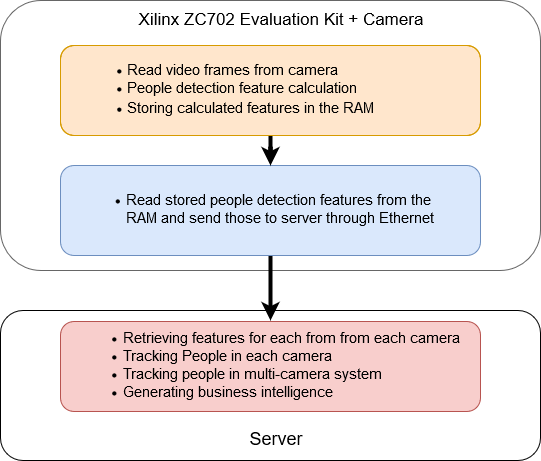
\includegraphics[width=9cm]{block_diagram.png}
\centering
\caption{Block diagram of the system}
\label{f1}
\end{figure}

\section{Overall Architecture}
Overall architecture of the implemented system is as follows. As explained earlier system consist of Zynq FPGA computation part and backend server computation part.
\begin{figure}[h]
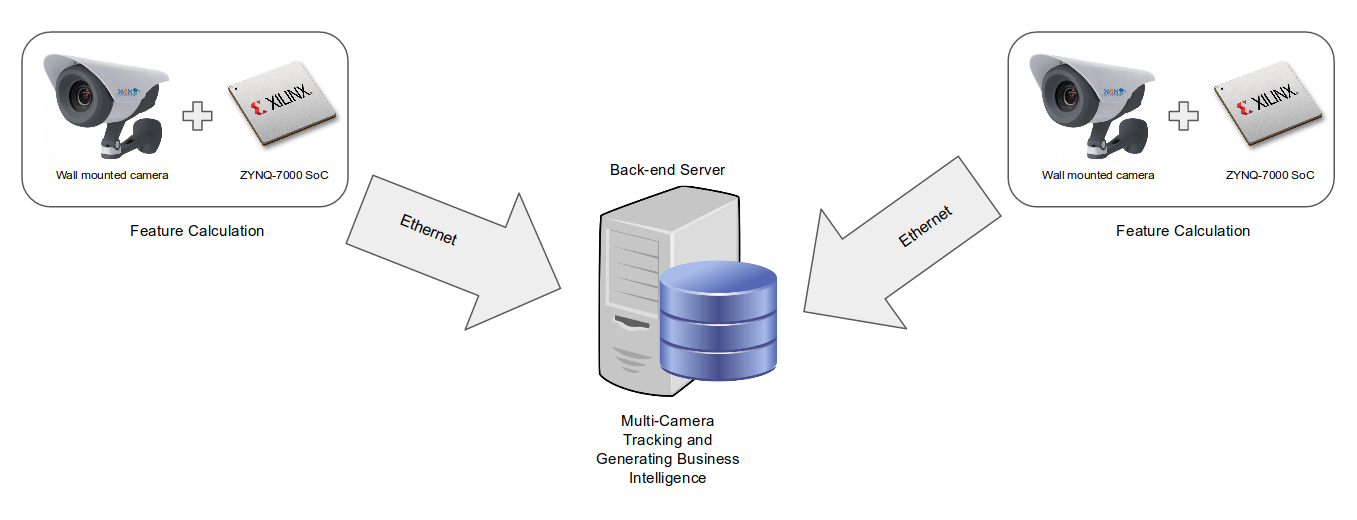
\includegraphics[width=10cm]{architecture.png}
\centering
\caption{Overall architecture of the system}
\label{f2}
\end{figure}

\section{Devices and Components Used}
\subsection{Xilinx ZC702 Evaluation Kit}
Based on the project requirements feature calculation for people detection will be done in these evaluation kits. This board is equipped with, 
\begin{itemize}
\item Zynq-7000 XC7z020 SoC, which includes a ARTIX-7 FPGA and two ARM CORTEX-A9 processors.
\item On-board 1GB DDR3 Component Memory
\item Hardware support for Ethernet, USB OTG, HDMI
\item Expand I/O with the FPGA Mezzanine Card (FMC) interface 
\end{itemize}
\begin{figure}[H]
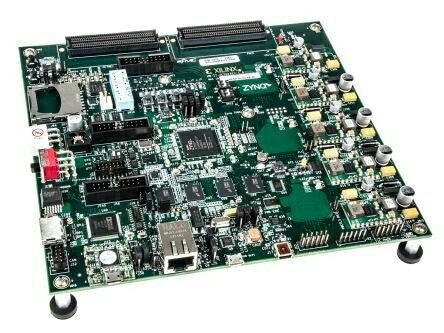
\includegraphics[width=8cm]{zc702.jpg}
\centering
\caption{Xilinx ZC702 Development Board}
\label{zc702}
\end{figure}

\section{Literature Review}
\par In this project we have to solve several challenging issues. The first part is people detection. There are various ways to achieve this. One way is to use a low level algorithm such as blob detection as used by Vicente, Alfredo Gardel, et al. \cite{1} in 2009.They have done background subtraction followed by contour detection to select head candidates for videos obtained using overhead cameras and they have implemented people detection part in a low cost FPGA (spartan3). 

\par Feature based methods are also another way to do people detection. In these methods a set of features are calculated around a window and some kind of machine learning algorithm is used to train a classifier that can classify each window into "contains a person" and "not contains a person". One such method is Histogram Oriented Gradient (HoG) based method suggested by Dalal, Navneet, and Bill Triggs. \cite{2} in 2005. A variation of HoG is implemented on FPGA by Negi, Kazuhiro, et al. \cite{3} in 2011.

\par Another approach that can be used for people detection is to utilize a neural network. If we can come up with a suitable neural network architecture, this method has the potential to outperform all the other methods mentioned earlier. Luckily there are open source implementations of such architectures available. One such architecture is given by Redmon, Joseph, et al. \cite{4} in 2016. Their work has made a huge leap in object detection space. Due to it's success their architecture is utilized by many people.

\par Other major challenge we have is people tracking based on our detections. There are many traditional approaches to this such as tracking using kalman filter and assigning detections to tracks using the Hungarian algorithm. But multi target tracking also can be formulated as a discrete-continuous optimization problem \cite{5}. Andriyenko, Anton, Konrad Schindler, and Stefan Roth \cite{5} in 2012 have considered data association as a discrete optimization problem with label costs. And they have posed trajectory estimation as a continuous fitting problem with closed form solutions. And there method has performed well on some known data sets.

\par Other major challenge that we face is, how to extend multiple target tracking into a multi camera framework. There are some research papers discussing this issue. Tang, Nick C., et al. \cite{6} in 2015 suggest a two pass regression framework to solve this challenge. First pass regressor predicts the people count based on the features calculated from intra-camera video frames. And then the second pass is based on the conflicts between the prediction derived from multiple views. They have formulated this as a transfer learning problem.

\par Yang, Tao, et al. \cite{7} in 2007 discusses another method to do this. In this approach first they do single camera tracking and they transform these tracked paths into a global coordinate system. Then by using their multi camera handoff algorithm, they can track people across multiple cameras. Here they calculate a match score for an object appearing in a camera under overlapping or nonoverlapping conditions for all tracks under all cameras. The track having the maximum score is selected.

\par By going through the available literature we were able to get an insight of the scope of our project. We identified some potential solutions for the challenges we have. And we also were able to identify some areas that we can make a novel contribution. One such contribution would be implementing people detection feature calculator (YOLO\cite{4} CNN, HoG or background subtraction based method) on FPGA. And the overall system architecture will also be an important contribution.

\chapter{Methodology}
Considering the project scope, this can be mainly divided into the following subsections. 
\begin{enumerate}
\item People Detection
\item Multi-Camera People Tracking
\item Business Intelligence Software
\end{enumerate}
 We will now consider each of these subsections and explain the methodologies used and also the alternative strategies considered.
\section{People Detection}
According to the project scope, idea was to calculate the features necessary for people detection in the FPGA. There are several techniques to achieve this task. They are, Background Subtraction, Histogram of Gradient (HoG) based People Detection and Convolutional Neural Networks.

\begin{table}[h]
\centering
\caption{People detection alternative strategies}
\label{t1}
\begin{tabular}{c|c|c|c|}
\cline{2-4}
\textbf{}                                                                                  & \textbf{\begin{tabular}[c]{@{}c@{}}Background \\ Subtraction\end{tabular}} & \textbf{\begin{tabular}[c]{@{}c@{}}Histogram of \\ Gradients\end{tabular}} & \textbf{\begin{tabular}[c]{@{}c@{}}Neural \\ Networks\end{tabular}}                                 \\ \hline
\multicolumn{1}{|c|}{Accuracy}                                                             & Low                                                                        & Average                                                                    & High                                                                                       \\ \hline
\multicolumn{1}{|c|}{\begin{tabular}[c]{@{}c@{}}Resource \\ Requirement\end{tabular}}      & Low                                                                        & Low                                                                        & High                                                                                       \\ \hline
\multicolumn{1}{|c|}{\begin{tabular}[c]{@{}c@{}}Implementation \\ Complexity\end{tabular}} & Low                                                                        & Average                                                                    & Very High                                                                                  \\ \hline
\multicolumn{1}{|c|}{Time Complexity}                                                      & Very Low                                                                   & Low                                                                        & High                                                                                       \\ \hline
\multicolumn{1}{|c|}{\begin{tabular}[c]{@{}c@{}}Existing \\ Implementations\end{tabular}}  & \begin{tabular}[c]{@{}c@{}}Lots of Papers \\ were found\end{tabular}       & \begin{tabular}[c]{@{}c@{}}Lots of Papers \\ were found\end{tabular}       & \begin{tabular}[c]{@{}c@{}}People Detection in \\ FPGA using \\ CNN is unique\end{tabular} \\ \hline
\end{tabular}
\end{table}

\subsection{Background Subtraction}
Background Subtraction is a fairly less complex algorithm which will yield a considerably less accuracy level. This method simply keeps a background model of the scene and updates its model using the upcoming image frames adaptively. 
\par Pros of this algorithm is that this can execute at much faster rate and also will require a less amount of resources in the FPGA.
\begin{figure}[H]
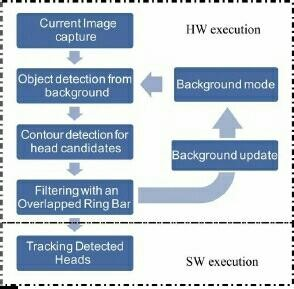
\includegraphics[width=8cm]{backg.jpg}
\centering
\caption{FPGA implementation of backgroung subtraction algorithm}
\label{backg}
\end{figure}

\subsection{Histogram of Gradients (HoG)}
HoG can be treated as one of the most popular and successful people detectors available. It is a type of a feature descriptor which is fairly simple to implement but also yields a fairly good accuracy. 
This approach uses a trained support vector machine to recognize HoG descriptors of people. This technique uses a sliding detection window which is moved in the image. HoG descriptors for each of these locations are calculated and then SVM classifier will classify these windows as either a person or not. Flow diagram of this algorithm is shown in figure \ref{hog}.
\begin{figure}[H]
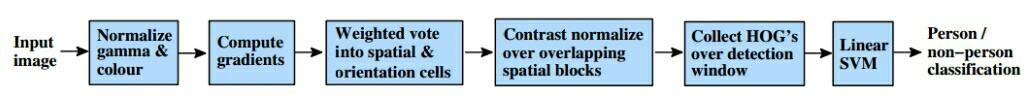
\includegraphics[width=14cm]{hog.jpg}
\centering
\caption{Flow diagram of HoG algorithm}
\label{hog}
\end{figure}
\subsection{Convolutional Neural Networks }
Convolutional neural networks which is a class of deep neural networks are mainly used in machine vision applications. People detection using CNN will yield a very high accuracy but also will be computationally complex. This in turn makes this algorithm the slowest but real time execution can be achieved with parallelization available in the FPGA.
\par This technique simply contains several layers of convolutions which are stacked together.
\begin{figure}[H]
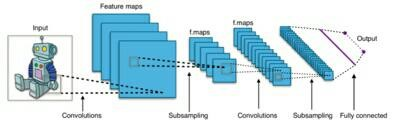
\includegraphics[width=10cm]{cnn.jpg}
\centering
\caption{Example of a CNN architecture}
\label{cnn}
\end{figure}
Considering the high accuracy we decided to use the CNN based approach.
Even in CNN there are several architectures we can use. Some of the architectures we considered are Deformable Parts Model (DPM), Fast RCNN and You Only Look Once (YOLO). 
\par DPM simply looks for all possible regions in the image to detect the objects. Faster RCNN will only do a selective search by first running the image through a region proposal network.
\par YOLO will do this task combined in one CNN network, so that the CNN output would be the centroids and the bounding boxes of the objects found. Therefore, currently YOLO is the fastest CNN architecture for people detection. 
\par Considering all these we selected YOLO for the task as it is the fastest and there was no earlier implementation of YOLO in an FPGA.
\begin{figure}[H]
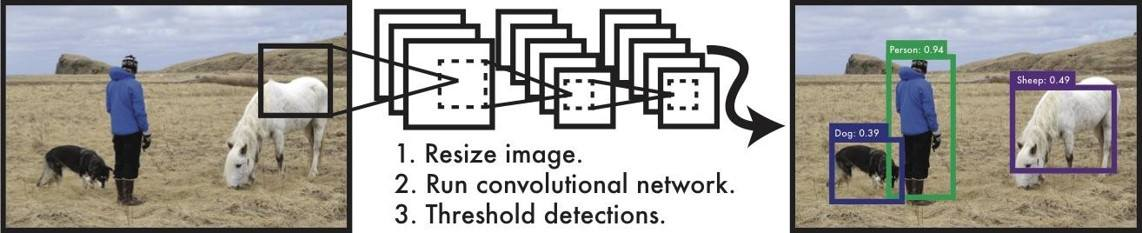
\includegraphics[width=10cm]{yolo.jpg}
\centering
\caption{YOLO\cite{4} CNN Architecture}
\label{yolo}
\end{figure}

\section{FPGA Hardware Design and Implementation}
\subsection{Design flow used for FPGA based System}
Following Xilinx tools were used to design the overall system on the FPGA,
\begin{enumerate}
\item Xilinx Vivado HLS
\item Xilinx Vivado
\item Xilinx Software Development Kit
\item Xilinx PetaLinux Software Development Kit
\end{enumerate}
Both 2014.4 and 2015.4 versions of above softwares were used in designing the system. Feature calculation IP core was first designed and implemented using C/C++ languages, as a function and then synthesized and converted to a RTL design using Vivado High Level Synthesis Tool. C simulation (functionality verification) and C/RTL co-simulation (RTL verification) was done to verify the design, before packaging the IP core using Vivado HLS.

\par Packaged IP core is then imported to Vivado tool for overall architecture design. Vivado’s block design feature was used to design the architecture.  After the system is designed, design verification was done, then overall system design is synthesized and RTL design and bit file (FPGA programmable file) was generated in Vivado. These generated files were then exported to used by the Xilinx SDK.

\par Generated RTL design was implemented on Xilinx ZC702 development board and tested using a C/C++ application code with Xilinx SDK. After the hardware designed is verified, designed is continued to the next phase, which is to generate Linux kernel boot files for the designed custom hardware and designing Linux drivers to control the designed IP core from Linux userspace.

\par RTL files generated from Vivado is then exported to a PetaLinux project for generating necessary boot files to boot Linux kernel on the custom hardware we designed. After enabling the required kernel drivers in kernel configuration and editing the device tree source files to include custom hardware peripherals in the kernel, PetaLinux project is built, which generates the required boot files. 

\par Above kernel files were used to boot Linux on ZC702 board. As the final step of the design flow, Linux userspace drivers were developed on top of the template driver generated by Vivado HLS for controlling the designed feature calculation IP core. 

\subsection{IP Core Hardware Design} 
IP core was designed to calculate the YOLO features. This was designed and synthesized using Xilinx Vivado High Level Synthesis (HLS) tool. Vivado HLS tool allows us to design the IP Core using C++ language, which will then be converted to RTL design by the tool.
\par YOLO architecture consists of 9 convolutional layers. This IP Core was designed in such a way that each layer will be executed separately given the inputs, weights and layer configurations for each layer.
\par IP Core consists of an AXI Master port which is connected to the SDRAM of ZC702 Kit. IP core will read the weights and layer inputs from the SDRAM through AXI Master port and the layer output after execution will also be written to the SDRAM through AXI Master interface. 
\par An AXILITE interface is present in order to feed the layer configuration into the IP Core. These configurations include width, height, input depth, output depth, ,kernel size, maxpooling, convolution, relu and padding.
\noindent Top design of the IP Core is shown in figure \ref{ip}.
\begin{figure}[H]
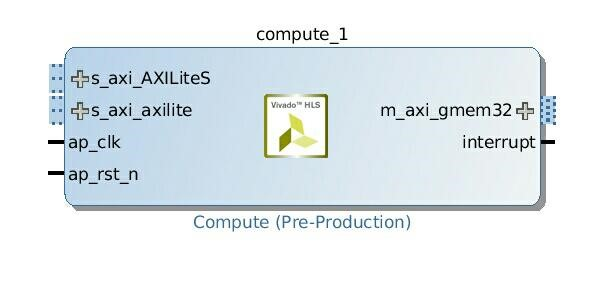
\includegraphics[width=10cm]{ip.jpg}
\centering
\caption{Block design of the designed feature calculation IP core}
\label{ip}
\end{figure}

\subsection{Overall Hardware Design}
Overall hardware design of the system was done using the Xilinx Vivado Design Suite. Overall hardware is fairly simple where the AXI Master port is connected to the ACP Port of Zynq Processing System. This is done since ACP port is connected to the SDRAM through Zynq PS. AXILITE port for providing the layer configurations was also connected to the Zynq PS through M\_AXI\_GP0 port.
\begin{figure}[H]
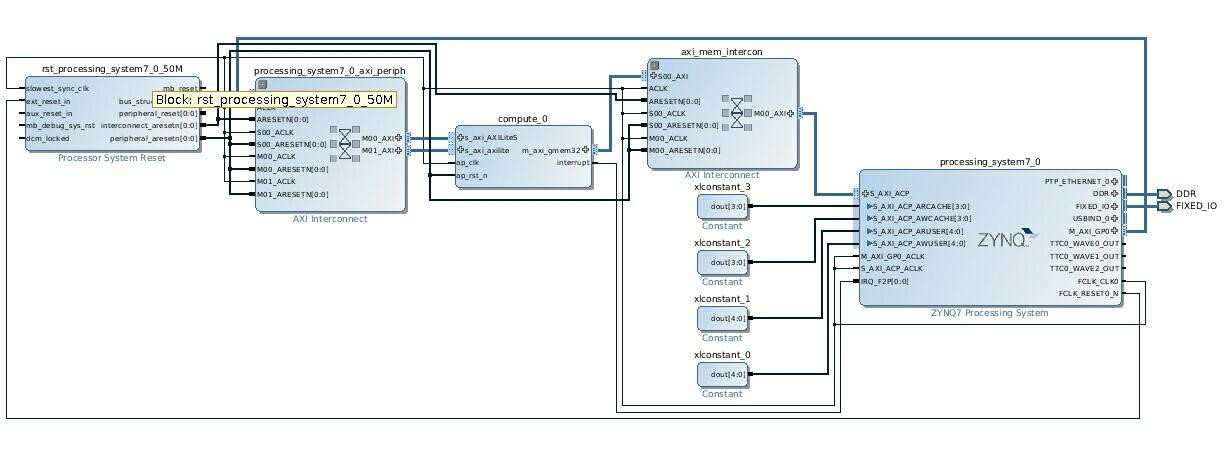
\includegraphics[width=15cm]{hardware.jpg}
\centering
\caption{Overall hardware architecture of the current designed system}
\label{hardware}
\end{figure}

\subsection{Linux Userspace Driver Development} 
According the scope of the project, overall system will be a linux based architecture. In order to achieve this task it is necessary to develop a linux driver to control our custom hardware. Therefore we developed a userspace input/output(UIO) driver to control the IP core and also the functionality of the custom hardware from Linux user space.
\begin{figure}[H]
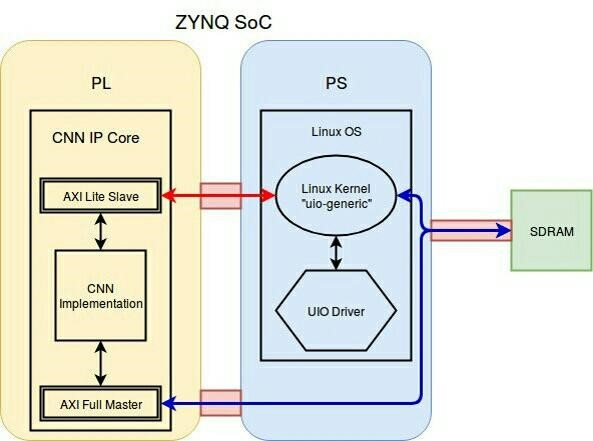
\includegraphics[width=11cm]{all.jpg}
\centering
\caption{Dataflow of the designed system on top of ZYNQ SoC}
\label{all}
\end{figure}
As shown in figure \ref{all}, developed UIO driver communicate with "uio-generic" kernel module which act as a portal between processing system(PS) partition and custom IP core we created in Programmable Logic(PL) partition of ZYNQ-7000 SoC. After configuration of the IP core is done, IP core is enabled using UIO driver. IP core then starts reading data from onboard RAM, processing data and storing back in the RAM. AXI Master port is used in these data transactions.  

\section{Multi Camera People Tracking}
Multi camera people tracking consist of tracking people through multiple cameras. In our design we consider some overlap between cameras. Due to availability of multiple viewpoints we can overcome occlusions up to some extent. In our design we have decomposed this into two tasks as follows.
\begin{itemize}
\item Single camera people tracking
\item Global people tracking based on single camera tracking
\end{itemize}
First of all we considered solving the first part: single camera people tracking.
\subsection{Single Camera People Tracking}
When it comes to object tracking, detection based tracking methods are the most popular. Multiple object tracking can be decomposed into two parts as, data association and target tracking. These multi object tracking algorithms can be divided into two categories. The first category relies on past frames to estimate the current state recursively. The second category allows for a certain latency and globally solves for all trajectories within a given time window. 
\par Since our system is to be run in real time, methods under first category are more appropriate for us. Under the first category we tried out Hungary algorithm followed by Kalman Filter based tracker for each object being tracked.  The block diagram of kalman filter based tracking system is shown below.
\subsubsection{\large Kalman Filter Based Tracking}
\begin{figure}[H]
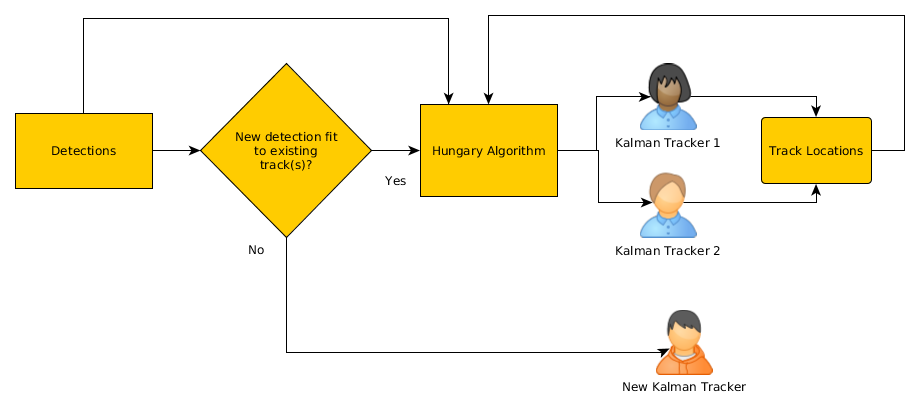
\includegraphics[width=10cm]{kalman_tracker.png}
\centering
\caption{Multiple people tracking using kalman filter}
\label{kalman}
\end{figure}
Here detection coordinates are fed to the backend tracking system by individual camera nodes (camera + zynq zc702). The next part of the algorithms calculates a cost matrix for detections vs existing tracks. For m detections and n tracks an entry of the cost matrix is given by equation \ref{eq1}.
\begin{equation}
\label{eq1}
c_{ij}= cost(detection\ i,\ track\ j)\ \  where\ i=1,...,m ;\ j=1,...,n
\end{equation}



Then detections having the minimum track cost lower than a threshold value are kept and detections exceeding the threshold value are initialized as new tracks. 
\par Here each track is a kalman filter. Dynamics model used in the kalman filter is a constant velocity model consisting of 6 state variables, namely { x coordinate, y coordinate, width, height, x velocity, y velocity} and 4 measurement variables, namely  { x coordinate, y coordinate, width, height}.
\par Detections to track assignments are done through the Hungarian algorithm. The Hungarian method is a combinatorial optimization algorithm that solves the assignment problem in polynomial time. Here the individual cost is the euclidean distance between x,y coordinates of the detection and the track. However this can be modified to include the width and height as well.
\par Tracks which have not been assigned to a detection within consecutive frames greater than a threshold value are simply deleted. \\
\noindent Although the kalman filter based tracking gives somewhat satisfactory results we are considering several improvements.
\begin{enumerate}
\item Using a particle filter.
\item Using a constant acceleration model.
\item Using Gaussian Mixture Models for track initialization.
\end{enumerate}
When we look at results we identified several weak points in our current tracking scheme. So we applied some modifications.
\subsubsection{\large Improvements for Kalman FIlter based Tracking}
In the data association step we have only considered the euclidean distance between detection and tracker coordinates for cost estimation. We improved the accuracy of data association by applying following modifications.\\\\
\textbf{Use gray level intensity histogram as a parameter in cost estimation}\\
We obtained the gray level intensity histogram for all the detection locations. And we included a histogram parameter in each tracker, where the histogram of the tracker is modified as follows at each assignment of a detection.
\begin{equation}
\label{eq2}
histogram_{tracker} = \alpha* histogram_{detection} + (1-\alpha) *histogram_{tracker}\        where\ 0\leq \alpha \leq1
\end{equation}
Then the correlation between the detection histogram and the tracker histogram is calculated and its inverse $(1/correlation coef.)$ is added to the cost. This makes our cost sensitive to the similarity of detection and tracker regions.\\\\
\textbf{Adding a penalty for the cost for high velocities in kalman filter state}\\
When the kalman filter tends to diverge the velocity value in the state vector becomes high. We can discard the kalman filter quickly by adding a penalty to the cost when the velocity is greater than a certain threshold.\\\\
\textbf{Tuning model parameters}\\
We have the following model parameters that must be properly tuned. Currently this is done in an ad hoc manner.
\begin{itemize}
\item Track Initialization Threshold - When the cost exceed this value a new tracker is initialized
\item Rejection Tolerance - When the count of a detection not being assigned to a tracker exceed this value the tracker is deleted
\item Velocity Threshold - Penalty is added to the cost when tracker velocity exceeds this value
\end{itemize}


\subsubsection{\large Discrete-Continuous Optimization for Multiple Target Tracking}
\begin{figure}[H]
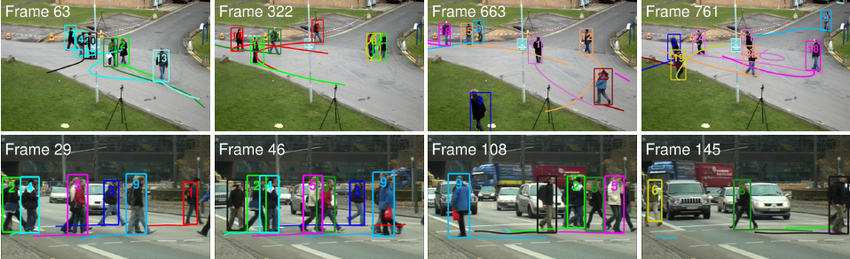
\includegraphics[width=10cm]{multi_peo.png}
\centering
\caption{Example frames from dicrete-continuous energy minimization approach \cite{5}}
\label{multi_peo}
\end{figure}
Under the second category we considered Discrete-Continuous Optimization for Multiple Target Tracking \cite{5}. Here Data association is performed using discrete optimization with label costs, yielding near optimality. Trajectory estimation is posed as a continuous fitting problem with a simple closed-form solution, which is used in turn to update the label costs. We can see from the results given in [5] (given in figure) that this method gives very good results.This method is more complex and computationally intensive than the kalman filter based approach. Since the kalman filter based approach gave satisfactory results we did not try to implement this method.

\subsection{Global Tracking}
Tracking via multiple cameras consist of 3 parts, people tracking per camera, correspondence estimation and global target tracking. There are 2 methods for correspondence estimation: homographic based methods and calibration based methods. Homography based methods rely on a set of matched features to calculate homographic transforms between images. Calibration based methods rely on a pre calculated model of the camera.
\par Out of these two methods we decided to use calibration based method because it can be easily integrated into single camera tracking algorithms that we considered. We only have to convert individual track coordinates into global coordinates and then perform global tracking.

\begin{figure}[H]
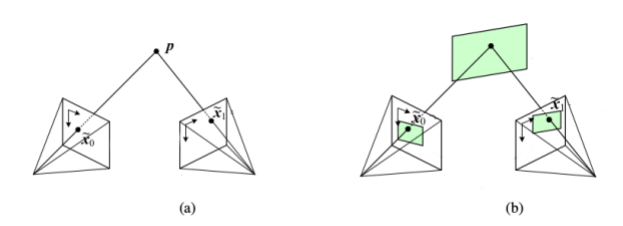
\includegraphics[width=10cm]{multi_cam.png}
\centering
\caption{Estimating global coordinates through calibrated cameras}
\label{multi_cam}
\end{figure}
When we have two calibrated cameras as shown in figure \ref{multi_cam}(a) the global 3D coordinates can be calculated from the image coordinates obtained from the two cameras, but we have to match the points across the cameras in order to do so. But if we limit our points to an arbitrary plane as shown in figure \ref{multi_cam}(b) we can obtain image coordinates projected to that plane. Suppose we limit our points to the ground plane. For this we can multiply the image coordinates (homogenous) by a homography matrix to obtain the ground plane coordinates.

\begin{equation}
\label{eq3}
x_g\ =\ Hx_{i}\ \    
\end{equation}   %check with dilin
In equation \ref{eq3}, H is a 3x3 homography matrix and $x_i,\ x_g$ are in homogeneous coordinates.
\begin{figure}[H]
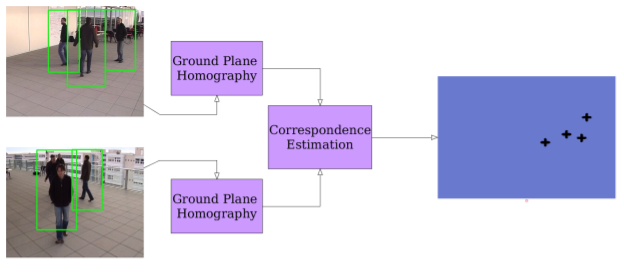
\includegraphics[width=12cm]{homo.png}
\centering
\caption{Multi-camera correspondence estimation}
\label{homo}
\end{figure}

\section{Communication among FPGA nodes and server}
The calculated features are sent to the server in order to track people and generate business intelligence. To enable communication among FPGA nodes and server we wrote two code structures in C++ and python. C++ client and server snippets connects ZYNQ SoC and the server backend whereas another C++ client and a python server connects the web interface. The block diagram of the communication structure is shown in the figure below.
\begin{figure}[H]
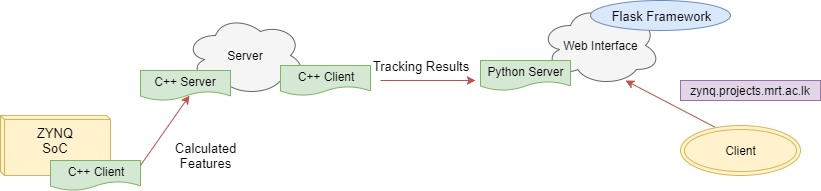
\includegraphics[width=10cm]{comm.png}
\centering
\caption{Data flow of the system}
\label{comm}
\end{figure}

\par The communications protocol used is UDP (User Datagram Protocol) to ensure low latency and reduce the processing overhead between communication nodes. Since this solution needs to be a real-time application, using TCP (Transmission Control Protocol) is not beneficial. One of the main reasons is dropping packets is desirable to waiting for packets delayed due to retransmission.
\par The retrieved features at the server backend are processed and multi camera tracking is done as discussed in the above section, which generates tracking results. That is ground plane coordinates of the individuals. This information is looped back to the server which is retrieved by a python server and redirects to a web interface written on the Flask framework. Flask web framework is based on python and it eases generating business intelligence data.
\par Clients can access the web interface through the URL ‘zynq.projects.mrt.ac.lk’ which directs to an internal server in ENTC. All the processing to generate tracking information is done in the said server. We have acquired a public IP in order to ensure that a client of this product can access the information on the go. Authentication will be provided so that unauthorized parties will not be able to access sensitive information.

\section{Business Intelligence Software}

Business intelligence software is designed as a website in order to allow access on the go. The web interface is based on Flask web Framework. As shown in the diagram in the above section. Flask which is based on Python is ideal for interactive real time user interface which showcases graphical data because Python provides a large graphics library ensuring an aesthetic design pleasing the eyes of the user and conveying the necessary information at the same time effectively. 

\par To retrieve real time data to the web server we have taken the RESTfull approach, which is based on REST API (Representational State Transfer Application Programming Interface).  REST is any interface between two systems which uses HTTP to obtain data and generate operations on those data in a variety of formats, such as XML and JSON. For our design the web page needs to be constantly updated without reloading the page. That is, the page that generates business intelligence (various graphs) needs to be drawn realtime. To ensure that the data is received realtime without a special user interaction such as pressing a button or refreshing the page we have integrated REST API and AJAX calls which provides the needed functionality. 

\par Another advantage of the RESTfull approach is that it enables data transfer in JSON object format. JSON is a text-based data format following JavaScript object syntax, which exists as a dictionary which is useful in transmitting data across networks.

\par The data is retrieved to the javascript with AJAX(Asynchronous JavaScript and XML) calls. AJAX calls are important in this scenario because data needs to be sent to the server in the background after the page has been loaded and update it without reloading the page. 


\chapter{Results}
\section{CNN IP Core Design}
As explained earlier CNN IP core to calculate YOLO features was designed using Vivado HLS. Its utilization estimates are as follows.
\begin{figure}[H]
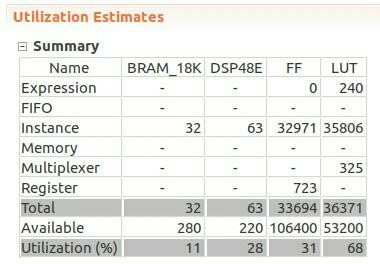
\includegraphics[width=10cm]{util.jpg}
\centering
\caption{Utilization table for YOLO CNN IP core on ZC702 board}
\label{util}
\end{figure}
Block diagram of a YOLO CNN ip core is shown in figure \ref{ip} and overall hardware architecture using this ip core is shown in figure \ref{hardware}.

\subsection{Discussion}
We were able to write Linux drivers for the hardware design and the results for the 1st layer of YOLO was verified in Linux. 
Though we got the anticipated output from the IP Core, initially the execution time for the 1st layer of YOLO was as high as 60 seconds. Ideally to obtain at least 5fps speed, first layer should finish executing in 20ms time. After few hardware optimizations we were able to reduce the execution time to 20 seconds with the maximum use of available resources in the FPGA.
We then assessed the reason for the high execution time. Reason was that the designed IP core access the DDR memory for weights and input data continuously one by one. 
\par As a solution to this issue, we decided to redesign the IP Core to use AXI Stream interface to acquire input data to the layers and use a Line Buffer based architecture for executing the convolution.

\section{Single Camera People Tracking}
Figure \ref{cam1} and figure \ref{cam2} shows people tracking results of two different cameras using only single camera tracking.
 \begin{figure}[H]
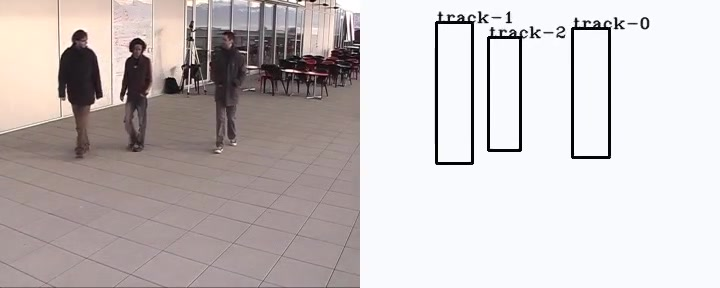
\includegraphics[width=10cm]{cam1.jpg}
\centering
\caption{Single camera people tracking results from camera 1}
\label{cam1}
\end{figure}
 \begin{figure}[H]
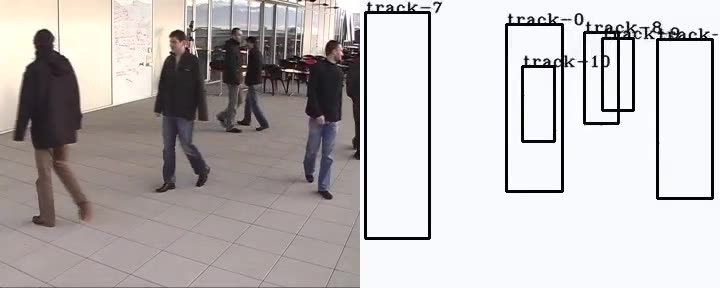
\includegraphics[width=10cm]{cam2.jpg}
\centering
\caption{Single camera people tracking results from camera 2}
\label{cam2}
\end{figure}
\subsection{Discussion}
Single view point tracking accuracy is very good if there are no occlusions. But when occlusions occur detection as well as data association becomes hard. As a result the tracking accuracy decreases under occlusions. In this situation assigning a detection to the corresponding kalman tracker becomes hard, and invalid assignments are performed, as a result the kalman filter diverges. But we can see that the algorithm is able to recover from such a situation by discarding that tracker and initiating a new tracker. We can make the data association more robust by using a particle filter based approach.

\subsection{Problems Faced}
One of the major issues in single camera tracking is solving the nonlinear data association problem. In our initial implementations we used euclidean distance between detection and tracker coordinates to perform data association. But when there are several detections in close vicinity invalid assignments are obtained. In order to overcome this we made several modifications to our original algorithm. 

\section{Global Tracking (Tracking using multiple cameras)}

 \begin{figure}[H]
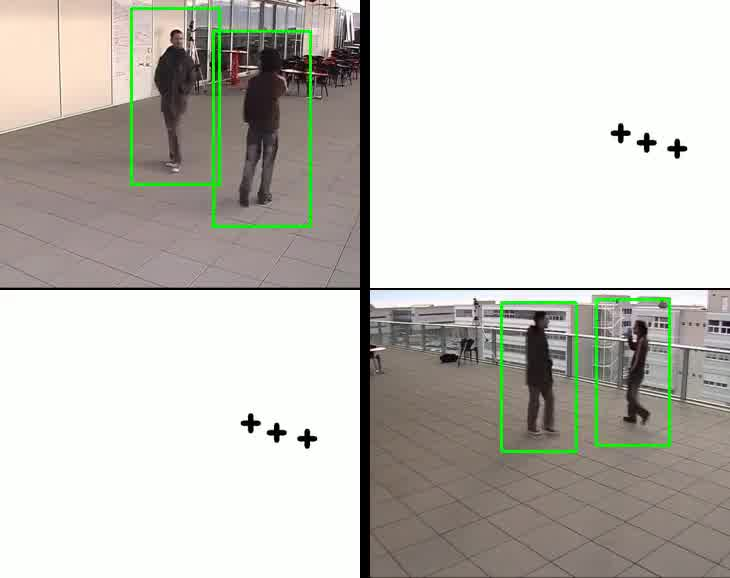
\includegraphics[width=12cm]{mul_cam1.jpg}
\centering
\caption{People tracking using multiple cameras and results mapped to a 2D plane}
\label{mul_cam1}
\end{figure}
 \begin{figure}[H]
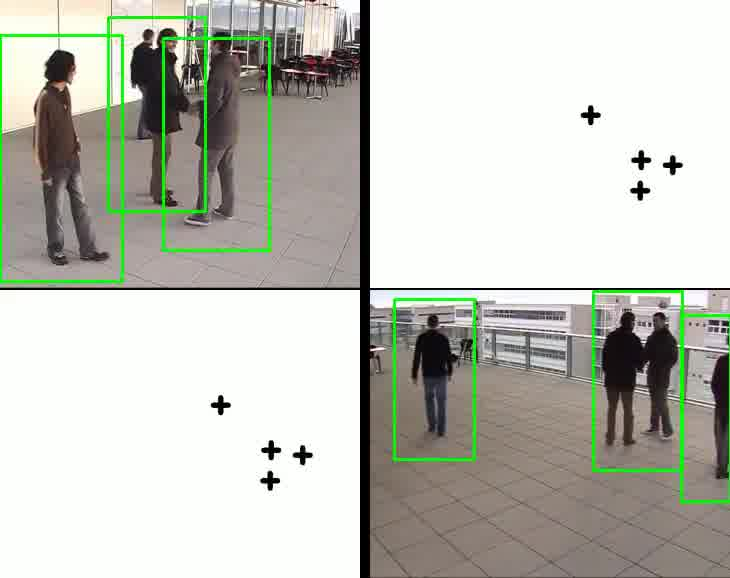
\includegraphics[width=12cm]{mul_cam2.jpg}
\centering
\caption{People tracking using multiple cameras and results mapped to a 2D plane (another two perspectives were used)}
\label{mul_cam2}
\end{figure}
\subsection{Discussion}
We have tested the multi camera correspondence estimation algorithm for 2 cameras based on detection coordinates. Above figures show results at 2 instances of the algorithm. We can see it gives satisfactory results up to some extent. But sometimes the correspondence estimation fails giving two points for the same person. Since this was based on detections directly this is acceptable. We can improve the results by performing global tracking using these location estimates.

\section{Business Intelligence Software}
The tracking information is sent by the C++ client as a JSON (JavaScript Object Notation) object. The structure of the json object is shown below.
\begin{figure}[H]
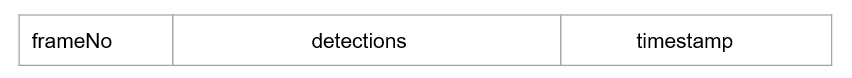
\includegraphics[width=12cm]{pak1.png}
\centering
\caption{JSON object structure}
\label{pak1}
\end{figure}

Inside the JSON object is a JSON array named detections containing (x,y) coordinates of the ground plane of separate individuals. For each person in the frame a row would be added to the detections array. This coordinates are used to map people to the store’s structure. Timestamp specifies the time at which the frame was captured.

\par To retrieve real time data to the server, we have employed REST API (Representational State Transfer Application Programming Interface).  

\par The following figure shows the structure that the AJAX call returns.
\begin{figure}[H]
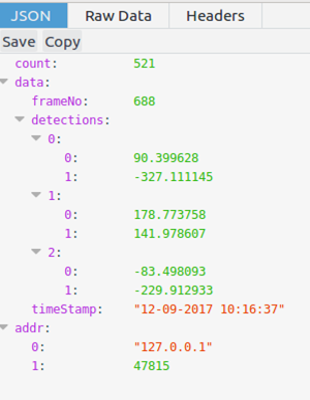
\includegraphics[width=8cm]{pak2.png}
\centering
\caption{Packet format which the AJAX call returns}
\label{pak2}
\end{figure}


Currently we have designed to two real time graphs.
\begin{itemize}
\item Store density graph - shows the number of people inside the store at real 	time.	
\item People 	coordinates graph – maps the ground plane coordinates of people at 	real time.
\end{itemize}

We are planning to implement the following graphs as well.
\begin{itemize}
\item Heat map 	of the store – highlights places where people stay mostly.
\item People 	tracking map - track an individual through the store.
\end{itemize}

\begin{figure}[H]
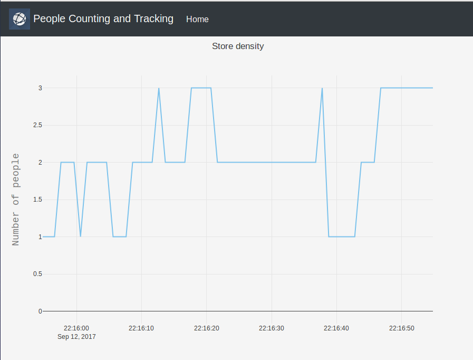
\includegraphics[width=8cm]{graph2.png}
\centering
\caption{Store Density graph}
\label{graph2}
\end{figure}

\begin{figure}[H]
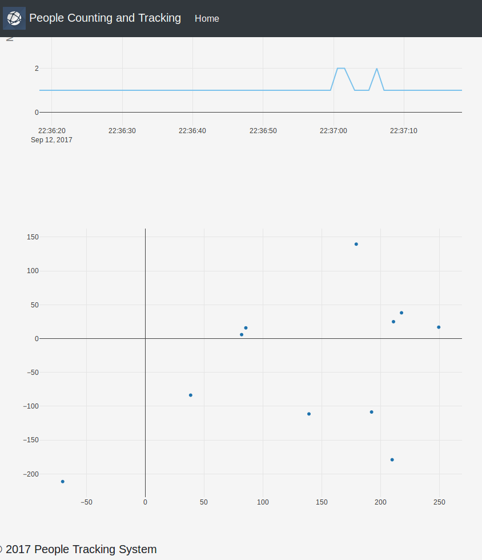
\includegraphics[width=8cm]{graph1.png}
\centering
\caption{People 	coordinates graph}
\label{grapg1}
\end{figure}








\newpage
%\section*{\textbf{References}}
\addcontentsline{toc}{section}{References}
\begin{thebibliography}{10}

\bibitem{1}
Vicente, Alfredo Gardel, et al. "Embedded vision modules for tracking and counting people." \textit{IEEE Transactions on Instrumentation and Measurement} 58.9 (2009): 3004-3011.

\bibitem{2}
Dalal, Navneet, and Bill Triggs. "Histograms of oriented gradients for human detection." Computer Vision and Pattern Recognition, 2005. CVPR 2005. \textit{IEEE Computer Society Conference on}. Vol. 1. IEEE, 2005.

\bibitem{3}
Negi, Kazuhiro, et al. "Deep pipelined one-chip FPGA implementation of a real-time image-based human detection algorithm." \textit{Field-Programmable Technology (FPT), 2011 International Conference on}. IEEE, 2011.

\bibitem{4}
Redmon, Joseph, et al. "You only look once: Unified, real-time object detection." \textit{Proceedings of the IEEE Conference on Computer Vision and Pattern Recognition}. 2016.

\bibitem{5}
Andriyenko, Anton, Konrad Schindler, and Stefan Roth. "Discrete-continuous optimization for multi-target tracking." \textit{Computer Vision and Pattern Recognition (CVPR), 2012 IEEE Conference on}. IEEE, 2012.

\bibitem{6}
Tang, Nick C., et al. "Cross-camera knowledge transfer for multiview people counting." \textit{IEEE Transactions on image processing} 24.1 (2015): 80-93.

\bibitem{7}
Yang, Tao, et al. "Robust people detection and tracking in a multi-camera indoor visual surveillance system." \textit{Multimedia and Expo, 2007 IEEE International Conference on}. IEEE, 2007.

\bibitem{8}
Flask.pocoo.org. (2017). Tutorial — Flask Documentation (0.12). [online] Available at: http://flask.pocoo.org/docs/0.12/tutorial/ [Accessed 6 Oct. 2017].

\bibitem{9}
Pythonprogramming.net. (2017). Python Programming Tutorials. [online] Available at: https://pythonprogramming.net/flask-registration-tutorial/ [Accessed 6 Oct. 2017].

\bibitem{10}
Flask-restful.readthedocs.io. (2017). Flask-RESTful — Flask-RESTful 0.3.6 documentation. [online] Available at: https://flask-restful.readthedocs.io/en/latest/ [Accessed 6 Oct. 2017].
\end{thebibliography}


\end{document}